\documentclass[11pt]{article}

\usepackage[margin=1.1in]{geometry}
\usepackage{amsmath,amssymb,amsthm}
\usepackage{tikz}
\usetikzlibrary{positioning}
\usepackage{booktabs}
\usepackage[colorlinks=true,linkcolor=blue!60!black,citecolor=blue!60!black]{hyperref}

\newtheorem{theorem}{Theorem}
\newtheorem{lemma}{Lemma}

\title{On the Convergence of Conflict-Free Replicated Documents}
\author{A.~Byrne \and L.~Okafor}
\date{July 2026}

\begin{document}
\maketitle

\begin{abstract}
Collaborative text editing requires that concurrent, uncoordinated edits at
distinct replicas converge to a single shared state without loss of intent.
We give a short, self-contained treatment of convergence for sequence CRDTs,
sketch why commutativity of concurrent operations suffices, and illustrate
the replica topology used by modern collaborative editors. This document
doubles as a demonstration manuscript: it exercises mathematics, a TikZ
figure, a table, and BibTeX citations in a single fast compile.
\end{abstract}

\section{Introduction}

Real-time collaborative editors must reconcile edits that were made
concurrently at different replicas. Operational transformation
\cite{ellis1989concurrency} approaches this by rewriting operations against
one another, while conflict-free replicated data types (CRDTs)
\cite{shapiro2011crdt} instead design the operations to commute. The
distinction matters operationally: commutative operations need no central
sequencer, so replicas may synchronize peer-to-peer or through any relay.

Typesetting systems have their own long history of correctness concerns
\cite{knuth1984texbook,lamport1994latex}; here we borrow only their notation.

\section{Convergence}

Let $\mathcal{O}$ be a set of operations and let $\parallel$ denote
concurrency of two operations. A replicated sequence is \emph{strongly
eventually consistent} when all replicas that have delivered the same set of
operations are in the same state.

\begin{theorem}[Convergence]\label{thm:conv}
If for all $a, b \in \mathcal{O}$ with $a \parallel b$ the effects commute,
\begin{equation}
  \mathrm{apply}(a) \circ \mathrm{apply}(b)
  \;=\;
  \mathrm{apply}(b) \circ \mathrm{apply}(a),
  \label{eq:commute}
\end{equation}
then any two replicas that deliver the same operation set reach equal states.
\end{theorem}

\begin{proof}[Proof sketch]
Delivery orders of the same set differ only by transpositions of concurrent
pairs; by \eqref{eq:commute} each transposition preserves the final state.
Causally ordered pairs are delivered in the same order at every replica by
assumption, so induction over the delivery sequence closes the argument.
\end{proof}

\begin{figure}[t]
\centering
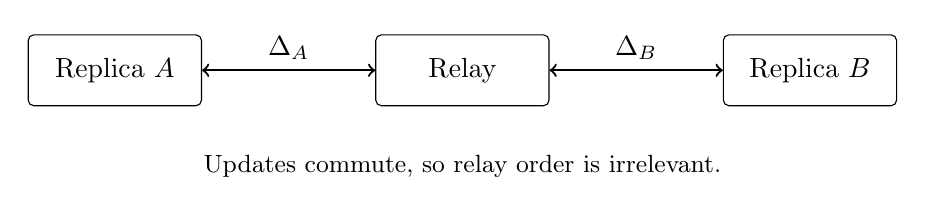
\begin{tikzpicture}[
  replica/.style={draw, rounded corners=2pt, minimum width=2.2cm, minimum height=0.9cm},
  node distance=1.4cm and 2.2cm
]
\node[replica] (a) {Replica $A$};
\node[replica, right=of a] (r) {Relay};
\node[replica, right=of r] (b) {Replica $B$};
\draw[<->, thick] (a) -- node[above] {$\Delta_A$} (r);
\draw[<->, thick] (r) -- node[above] {$\Delta_B$} (b);
\node[below=0.5cm of r] {\small Updates commute, so relay order is irrelevant.};
\end{tikzpicture}
\caption{Replicas exchanging commutative updates through an untrusted relay.}
\label{fig:topology}
\end{figure}

\section{Cost model}

Table~\ref{tab:cost} summarizes asymptotic costs per edit for common designs,
where $n$ is document length and $c$ the number of concurrent editors.

\begin{table}[htbp]
\centering
\begin{tabular}{lccc}
\toprule
Design & Apply & Merge & Metadata \\
\midrule
OT (central) & $O(1)$ & $O(c)$ & $O(1)$ \\
List CRDT & $O(\log n)$ & $O(\log n)$ & $O(n)$ \\
\bottomrule
\end{tabular}
\caption{Per-edit costs; constants matter more than asymptotics in practice.}
\label{tab:cost}
\end{table}

\section{Related work}

Operational transformation dominated the first two decades of collaborative
editing research and practice \cite{ellis1989concurrency}; its correctness
proofs are notoriously delicate because transformation functions must satisfy
convergence properties under arbitrary interleavings. CRDTs shift that burden
from the algorithm to the data type \cite{shapiro2011crdt}: the proof
obligation is discharged once, at design time, rather than re-examined for
every server implementation.

A related line of work concerns \emph{intention preservation}: convergence
guarantees replicas agree, not that they agree on something sensible. List
CRDTs address the common anomalies (interleaving of concurrent runs of text,
resurrection of deleted ranges) with ordering metadata; the residual cases
are rare enough in interactive editing that user-visible anomalies are
dominated by presentation-layer issues rather than by the merge itself.

\section{Conclusion}

Commutativity (Theorem~\ref{thm:conv}) is the whole trick: once concurrent
operations commute, convergence is a property of the data type rather than of
the network. Everything else — presence, cursors, history — is engineering.

\appendix

\section{A lemma on causal delivery}

\begin{lemma}
If delivery respects causal order, then for any operation $o$ every
operation $o'$ with $o' \rightarrow o$ (happens-before) is applied before
$o$ at every replica, and Theorem~\ref{thm:conv} applies to the remaining
concurrent pairs.
\end{lemma}

\begin{proof}
Immediate from the definition of causal delivery: the delivery order at each
replica is a linear extension of the happens-before partial order, and any
two linear extensions of the same partial order differ by transpositions of
incomparable (concurrent) elements only.
\end{proof}

\bibliographystyle{plain}
\bibliography{references}

\end{document}
